\section{Unknown Samples}
In this part we got 5 samples of ashe from leaves and pines, from eastern europe.
Of these samples, we took the gamma spectrum with the HPGE detector and compared them with a refference sample.
The sample contains radioactive $^{137}$Cs which is supossed to be contained in the ashe, because of the Chernobyl nuclear accident.
In the following we compare the acitivty of $^{137}$Cs from the ashe with the refference.
From all spectra we substracted the background radiation.

In Fig. \ref{cher_samples} we can see the spectrum of the refference and the samples.
\begin{figure}[h]
\begin{subfigure}{.5\textwidth}
  \centering
  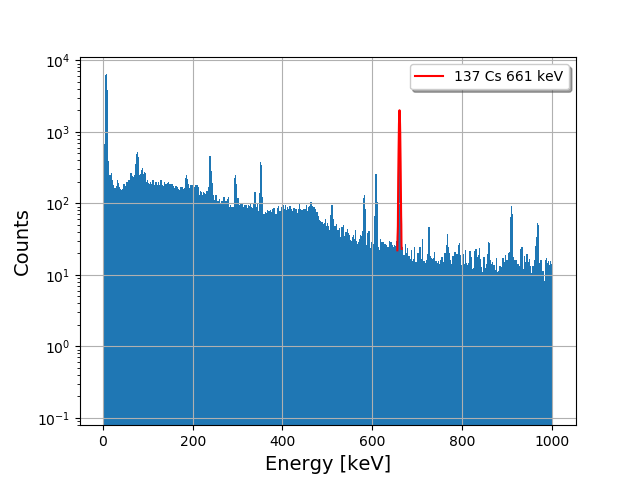
\includegraphics[width=.9\linewidth]{pictures/cher_ref.png}
  \caption{Reference sample}
\end{subfigure}%
\begin{subfigure}{.5\textwidth}
  \centering
  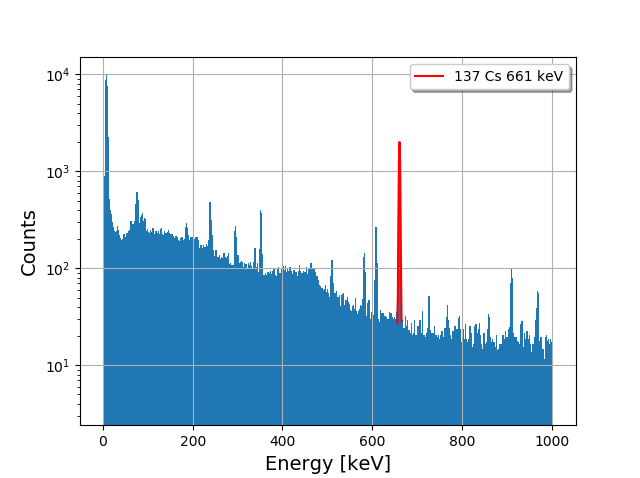
\includegraphics[width=.9\linewidth]{../plots/PP34R1_1.png}
  \caption{Sample $PP34R1\_1$}
\end{subfigure}%
 \vskip\baselineskip
\begin{subfigure}{.5\textwidth}
  \centering
  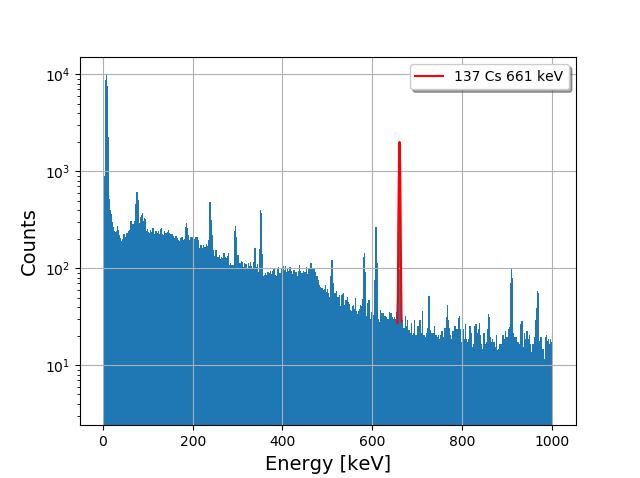
\includegraphics[width=.9\linewidth]{../plots/PP5PR1_2.png}
  \caption{Sample $PP5PR1\_2$}
\end{subfigure}%
\begin{subfigure}{.5\textwidth}
  \centering
  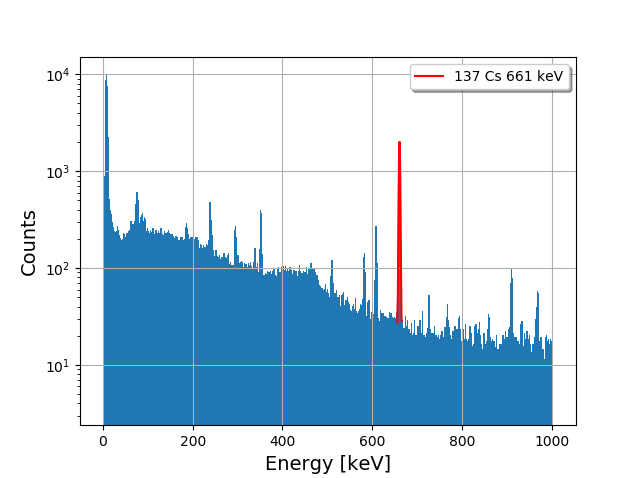
\includegraphics[width=.9\linewidth]{../plots/PP63R1_3.png}
  \caption{Sample $PP63R1\_3$}
\end{subfigure}%
 \vskip\baselineskip
\begin{subfigure}{.5\textwidth}
  \centering
  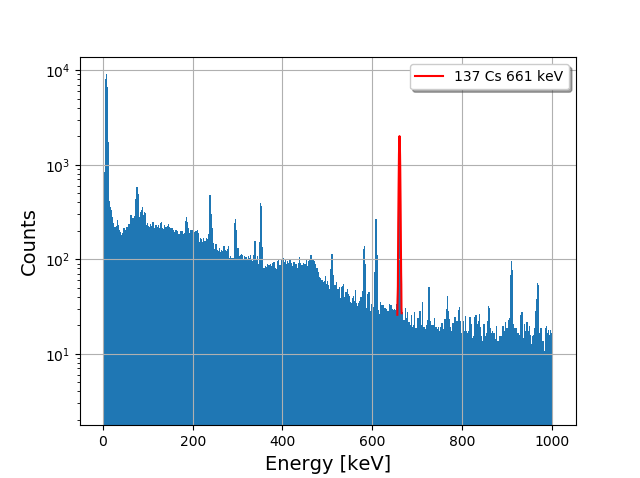
\includegraphics[width=.9\linewidth]{../plots/PP84R2_4.png}
  \caption{Sample $PP84R2\_4$}
\end{subfigure}%
\begin{subfigure}{.5\textwidth}
  \centering
  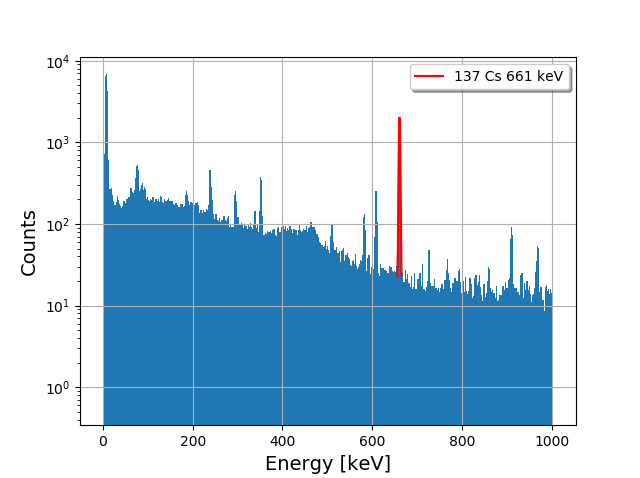
\includegraphics[width=.9\linewidth]{../plots/PPACR2_5.png}
  \caption{Sample $PPACR2\_5$}
\end{subfigure}%
\caption{gamma spectra of the measured samples}
\label{cher_samples}
\end{figure}
Measurement time was around 3h.
In every samples we can clearly  see a  $^{137}$Cs peak, together with smaller peaks.
Some of these smaller peaks might come from natural occuring isotopes, while some might result from the Chernobyl accident too.
For this analysis we will concentrate on $^{137}$Cs.

From the peaks we calculated the measured acitivty again as:
\begin{equation}
A_i = \frac{N_{obs}}{t_{live} \eta (E_i) P}
\end{equation}
The observed counts $N_{obs}$ were this time calculated as:
\begin{equation}
N_{obs} = \frac{I \sigma \sqrt{2 \cdot \pi}}{b}
\end{equation}
With the binwidth $b = 0.4$ to compensate the change of binwidth on the energy scale.
For the analysis we than took the ration $\frac{A_i}{A_0}$ with the activity of the reference $A_0$ and the activity of the samples $A_i$.
The results can be seen in Tab. \ref{cher_results}.
The uncertainties were calculated from the uncertainty of $N_{obs}$ and $\eta$.

\begin{table}[h]
\centering
\begin{tabular}{c |c | c }
\hline
Sample & A [Bq] & $\frac{A}{A_0}$ \\
\hline
Reference & $8.1 \pm 1.2   $ & $1$ \\
$PP34R1\_1  $& $113.7 \pm 1.3$ & $14.1 \pm 4.3$ \\
$PP5PR1\_2  $& $114.4 \pm 1.3$ & $14.2 \pm 4.4$ \\
$PP63R1\_3  $& $106.6 \pm 1.3$ & $13.2 \pm 4.0$ \\
$PP84R2\_4  $& $36.2 \pm 1.3  $ & $4.5 \pm 1.4$ \\
$PPACR2\_5 $& $14.4 \pm 1.3  $ & $1.8 \pm 1.4$ \\
\hline
\end{tabular}
\label{cher_results}
\end{table}
Every measured sample has a higher activity than the reference sample.
The lowest acitivity is with sample $PPACR2\_5$, which has nearly double the acitivity of the reference source.
Three of the samples ($PP34R1\_1, PP5PR1\_2 \text{and} PP63R1\_3$) have an activity more than ten times higher, which could mean, that these contain a considerable amount of radioactive  $^{137}$Cs.
